\documentclass[lang=cn,11pt,a4paper]{elegantpaper}
\DeclareMathOperator*{\minimize}{minimize}
\DeclareMathOperator*{\maximize}{maximize}
\DeclareMathOperator*{\argmin}{argmin}
\DeclareMathOperator*{\argmax}{argmax}
\title{线性收缩 Ridge}
\author{ 殷润轩   \\ Sun Yat-sen University }
\institute{数学学院(珠海) \LaTeX{} }
\version{1.0}
\date{\zhtoday}

\DeclareMathSizes{12}{14}{10}{8} % (正文大小, 行间公式, 上标和下标, 附加大小)

\usepackage{array}
\usepackage{enumitem}
\usepackage{codehigh}
\usepackage{amsmath} % 导入amsmath宏包,提供align环境
\usepackage{multirow}
\usepackage{array}
\usepackage{diagbox}
\usepackage{graphicx}
\usepackage{caption}
\usepackage{float}
\usepackage{comment}
\usepackage{amsmath, amssymb, amsthm}
\usepackage{tcolorbox}
\usepackage{bm} % 加载 bm 宏包
\usepackage{tikz}
\tcbuselibrary{theorems}

% 定义带黑色边框的定理环境

\newcommand{\ccr}[1]{\makecell{{\color{#1}\rule{1cm}{1cm}}}}

\begin{document}
\maketitle
\begin{abstract}

\keywords{收缩}
\end{abstract}
\section{前置数学知识}
\subsection{范数}
范数是定义在向量空间上的函数,用于衡量向量的大小。在机器学习中,常用的范数包括 \( L^1 \) 范数和 \( L^2 \) 范数。给定 \( n \) 维向量 \( x = (x_1, x_2, \dots, x_n) \),其 \( L^1 \) 范数和 \( L^2 \) 范数分别定义为:
\begin{equation}
\| x \|_1 = \sum_{i=1}^n |x_i|, \quad \| x \|_2 = \sqrt{\sum_{i=1}^n x_i^2}
\end{equation}
\( L^1 \) 范数衡量向量元素绝对值之和,常用于稀疏模型;\( L^2 \) 范数衡量向量元素平方和的平方根,常用于最小二乘模型。
\subsection{向量求导}

\begin{theorem}{方向导数与梯度的关系}
    若函数 \( f: \mathbb{R}^n \to \mathbb{R} \) 是 \( C^1 \) 类(一阶连续可导),则方向导数满足:
    \begin{equation}
    Df(\mathbf{x})[\mathbf{v}] = \mathbf{v}^T \nabla f(\mathbf{x}),
    \end{equation}
    其中 \( \mathbf{v} \) 是方向向量,\( \nabla f(\mathbf{x}) \) 是梯度。
\end{theorem}
\begin{proof}
        \textbf{方向导数的定义}:
        \begin{equation}
        Df(\mathbf{x})[\mathbf{v}] = \lim_{h \to 0} \frac{f(\mathbf{x} + h\mathbf{v}) - f(\mathbf{x})}{h}.
        \end{equation}
        \textbf{一阶泰勒展开}:对 \( f(\mathbf{x} + h\mathbf{v}) \) 展开:
        \begin{equation}
        f(\mathbf{x} + h\mathbf{v}) \approx f(\mathbf{x}) + h \nabla f(\mathbf{x})^T \mathbf{v} + o(h).
    \end{equation}
        代入定义式得:
        \begin{equation}
        Df(\mathbf{x})[\mathbf{v}] = \nabla f(\mathbf{x})^T \mathbf{v} =\mathbf{v}^T \nabla f(\mathbf{x}).
    \end{equation}
\end{proof}

    
    
    % ------------------------- 定理13 -------------------------
\begin{theorem}{Hessian矩阵与梯度方向导数的关系}
    若函数 \( f: \mathbb{R}^n \to \mathbb{R} \) 是 \( C^2 \) 类(二阶连续可导),则:
    \begin{equation}
    \nabla^2 f(\mathbf{x}) \cdot \mathbf{v} = D(\nabla f(\mathbf{x}))[\mathbf{v}],
    \end{equation}
    其中 \( \nabla^2 f(\mathbf{x}) \) 是Hessian矩阵,\( D(\nabla f(\mathbf{x}))[\mathbf{v}] \) 表示梯度沿方向 \( \mathbf{v} \) 的方向导数。
\end{theorem}
\begin{proof}
        \textbf{梯度的方向导数}:梯度 \( \nabla f(\mathbf{x}) \) 的方向导数为:
        \begin{equation}
        D(\nabla f(\mathbf{x}))[\mathbf{v}] = \begin{bmatrix}
            D(\partial_{x_1} f)[\mathbf{v}] \\
            \vdots \\
            D(\partial_{x_n} f)[\mathbf{v}]
        \end{bmatrix}.
        \end{equation}
        \textbf{Hessian矩阵的作用}:由于 \( \nabla^2 f(\mathbf{x}) = \mathbf{J}(\nabla f(\mathbf{x})) \),直接计算得:
        \begin{equation}
        D(\nabla f(\mathbf{x}))[\mathbf{v}] = \nabla^2 f(\mathbf{x}) \cdot \mathbf{v}.
        \end{equation}
\end{proof}

\begin{example}
我们需要找到函数 \( f(x) = \frac{1}{2} x^T A x \) 的梯度(gradient)和Hessian矩阵(Hessian matrix)。这里 \( x \) 是一个向量,\( A \) 是一个矩阵。
\end{example}


方向导数 \( D f(x)[v] \) 表示函数 \( f \) 在点 \( x \) 处沿方向 \( v \) 的变化率,定义为:
\begin{equation}
D f(x)[v] = \lim_{t \to 0} \frac{f(x + t v) - f(x)}{t}
\end{equation}
根据梯度的性质,方向导数也可以表示为:
\begin{equation}
D f(x)[v] = v^T \nabla f(x)
\end{equation}
将 \( f(x + t v) \) 展开:
\begin{equation}
f(x + t v) = \frac{1}{2} (x + t v)^T A (x + t v)
\end{equation}
展开后得到:
\begin{equation}
f(x + t v) = \frac{1}{2} x^T A x + \frac{t}{2} x^T A v + \frac{t}{2} v^T A x + \frac{t^2}{2} v^T A v
\end{equation}
将展开后的表达式代入方向导数的定义:
\begin{equation}
D f(x)[v] = \lim_{t \to 0} \frac{\frac{1}{2} x^T A x + \frac{t}{2} x^T A v + \frac{t}{2} v^T A x + \frac{t^2}{2} v^T A v - \frac{1}{2} x^T A x}{t}
\end{equation}
化简后得到:
\begin{equation}
D f(x)[v] = \frac{1}{2} x^T A v + \frac{1}{2} v^T A x
\end{equation}
由于矩阵乘法的转置性质 \( v^T A x = x^T A^T v \),如果 \( A \) 是对称矩阵(即 \( A = A^T \)),则:
\begin{equation}
\frac{1}{2} x^T A v + \frac{1}{2} v^T A x = v^T A x
\end{equation}
根据方向导数的表达式 \( D f(x)[v] = v^T \nabla f(x) \),我们得出:
\begin{equation}
\nabla f(x) = A x
\end{equation}
通过方向导数的定义和矩阵运算的性质,我们推导出函数 \( f(x) = \frac{1}{2} x^T A x \) 的梯度为 \( \nabla f(x) = A x \)。Hessian矩阵通常为 \( A + A^T \),如果 \( A \) 是对称矩阵,则 Hessian 矩阵为 \( 2A \)。

\section{矩阵求导}


\subsection{矩阵求导的定义}
设标量函数 \( f: \mathbb{R}^{m \times n} \to \mathbb{R} \),其关于矩阵 \(\bm{X} \in \mathbb{R}^{m \times n}\) 的导数为:
\[
\frac{\partial f}{\partial \bm{X}} = \begin{bmatrix}
\frac{\partial f}{\partial x_{11}} & \cdots & \frac{\partial f}{\partial x_{1n}} \\
\vdots & \ddots & \vdots \\
\frac{\partial f}{\partial x_{m1}} & \cdots & \frac{\partial f}{\partial x_{mn}} 
\end{bmatrix} \in \mathbb{R}^{m \times n}.
\]

\subsection{典型公式}
\begin{enumerate}
    \item \textbf{线性函数的导数}:
    \[
    f(\bm{X}) = \mathrm{tr}(\bm{A}^\top \bm{X}), \quad \frac{\partial f}{\partial \bm{X}} = \bm{A}.
    \]
    
    \item \textbf{二次型的导数}(\(\bm{X}\)对称时):
    \[
    f(\bm{X}) = \mathrm{tr}(\bm{X}^\top \bm{A} \bm{X}), \quad \frac{\partial f}{\partial \bm{X}} = 2\bm{A}\bm{X}.
    \]
    
    \item \textbf{行列式的导数}(\(\bm{X}\)可逆时):
    \[
    f(\bm{X}) = \det(\bm{X}), \quad \frac{\partial f}{\partial \bm{X}} = \det(\bm{X}) \cdot (\bm{X}^{-1})^\top.
    \]
    
    \item \textbf{迹的导数}:
    \[
    f(\bm{X}) = \mathrm{tr}(\bm{A} \bm{X} \bm{B}), \quad \frac{\partial f}{\partial \bm{X}} = \bm{A}^\top \bm{B}^\top.
    \]
    
    \item \textbf{矩阵逆的导数}:
    \[
    \frac{\partial \bm{X}^{-1}}{\partial \bm{X}} = -\bm{X}^{-\top} \otimes \bm{X}^{-\top}.
    \]
\end{enumerate}

\section{数学总结}
\begin{equation}
    f(\mathbf{x}) = \mathbf{a}^\top \mathbf{x}, \quad 
    \frac{\partial f}{\partial \mathbf{x}} = \mathbf{a}
\end{equation}
当矩阵\(\mathbf{A}\)对称时
\begin{equation}
    f(\mathbf{x}) = \mathbf{x}^\top \mathbf{A} \mathbf{x}, \quad 
    \frac{\partial f}{\partial \mathbf{x}} = 2\mathbf{A}\mathbf{x}
\end{equation}
若 \(\mathbf{A}\) 不对称:
\begin{equation}
    \frac{\partial f}{\partial \mathbf{x}} = (\mathbf{A} + \mathbf{A}^\top) \mathbf{x}
\end{equation}



\section{实际观测中的最小二乘问题}
假设物理量 \( y \) 与 \( n \) 个自变量 \( x_1, x_2, \dots, x_n \) 满足线性关系:
\begin{equation}
y = \lambda_1 x_1 + \lambda_2 x_2 + \cdots + \lambda_n x_n,
\end{equation}
通过 \( m \) 次观测(\( m > n \))得到超定方程组。需找到系数 \( \lambda_1, \dots, \lambda_n \) 最小化残差平方和。
\begin{equation}
\min_{\lambda_1, \dots, \lambda_n} \sum_{j=1}^m \left( y^{(j)} - \sum_{i=1}^n \lambda_i x_i^{(j)} \right)^2.
\end{equation}
设计矩阵 \( X \)、观测向量 \( y \)、系数向量 \( \lambda \) 定义如下:
\[
X = \begin{bmatrix}
x_1^{(1)} & \cdots & x_n^{(1)} \\
\vdots & \ddots & \vdots \\
x_1^{(m)} & \cdots & x_n^{(m)}
\end{bmatrix},\quad
y = \begin{bmatrix} y^{(1)} \\ \vdots \\ y^{(m)} \end{bmatrix},\quad
\lambda = \begin{bmatrix} \lambda_1 \\ \vdots \\ \lambda_n \end{bmatrix}.
\]
\subsection{目标函数与解析解}
在线性回归中,目标是最小化预测值与实际值之间的平方误差。这可以通过最小二乘法来实现,其数学表达式如下:
\begin{equation}
\min_{\lambda} \| y - X \lambda \|_2^2
\end{equation}
其中,\( y \) 是观测值向量,\( X \) 是设计矩阵(包含自变量),\( \lambda \) 是回归系数向量。
为了找到使目标函数最小的 \( \lambda \),我们对目标函数关于 \( \lambda \) 求导并令其等于零。目标函数的导数为:
\begin{equation}
\nabla_{\lambda} \| y - X \lambda \|_2^2 = -2 X^\top (y - X \lambda)
\end{equation}
将其设为零向量:
\begin{equation}
-2 X^\top (y - X \lambda) = 0
\end{equation}
化简得到正规方程(Normal Equation):
\begin{equation}
X^\top X \lambda = X^\top y
\end{equation}
如果 \( X^\top X \) 是可逆的,那么可以直接解出 \( \lambda \):
\begin{equation}
\lambda = (X^\top X)^{-1} X^\top y
\end{equation}
这就是线性回归的最小二乘解。它表示在给定设计矩阵 \( X \) 和观测值 \( y \) 的情况下,使得预测误差平方和最小的回归系数 \( \lambda \)。
\subsection{梯度下降法求数值解}
梯度下降法是一种迭代优化算法,用于寻找目标函数的最小值。其基本思想是沿着目标函数梯度的反方向更新模型参数,逐步逼近最优解。
目标函数为:
\begin{equation}
J(\lambda) = \frac{1}{2} \| y - X \lambda \|_2^2
\end{equation}
梯度为:
\begin{equation}
\nabla J(\lambda) = -X^\top (y - X \lambda)
\end{equation}
初始化回归系数向量 \( \lambda \),然后在每次迭代中按照以下规则更新:
\begin{equation}
\lambda^{(k+1)} = \lambda^{(k)} - \eta \nabla J(\lambda^{(k)})
\end{equation}
其中,\( \eta \) 是学习率,控制每次更新的步长。以下是算法流程:
\begin{enumerate}
    \item 初始化回归系数向量 \( \lambda \) 为零向量或随机小值。
    \item 计算当前 \( \lambda \) 对应的目标函数梯度 \( \nabla J(\lambda) \)。
    \item 按照学习率 \( \eta \) 更新 \( \lambda \)。
    \item 重复步骤2和3,直到满足收敛条件(如梯度范数小于某个阈值或目标函数变化小于某个阈值)。
\end{enumerate}
\par
学习率 \( \eta \) 是梯度下降法中的一个重要超参数。学习率过大可能导致算法发散,过小则可能导致收敛速度过慢。通常通过试验或使用学习率调度策略来选择合适的学习率。
梯度下降法在目标函数为凸函数时能够保证收敛到全局最优解。对于线性回归的最小二乘问题,目标函数是凸二次函数,因此梯度下降法能够可靠地收敛到最优解。
\par
代码在code中已经实现。
\section{带罚项的模型理论与性质}
当矩阵 \( X^\top X \) 不可逆或其行列式接近于零时,会导致以下问题和后果:
\subsection{矩阵不可逆的原因}
矩阵 \( X^\top X \) 的行列式为零时,矩阵是奇异的(不可逆),这通常发生在以下情况:
\begin{itemize}
    \item 自变量之间存在多重共线性(特征之间高度相关)。
    \item 自变量的数量多于样本量。
    \item 矩阵的列向量线性相关。
\end{itemize}

\subsection{不可逆带来的问题}
在普通最小二乘法(OLS)中,参数估计公式为:
\begin{equation}
\lambda = (X^\top X)^{-1} X^\top y
\end{equation}
需要矩阵 \( X^\top X \) 可逆。如果矩阵不可逆,参数无法直接计算。此外,行列式接近零时,矩阵的条件数较大,导致数值计算不稳定,可能引发误差放大。

\subsection{引入惩罚项的作用}
为了处理矩阵不可逆或行列式接近零的问题,可以引入惩罚项(如岭回归中的L2正则化)。惩罚项通过在损失函数中添加正则化项,使得矩阵 \( X^\top X \) 变为:
\begin{equation}
X^\top X + \lambda I
\end{equation}
其中 \( \lambda \) 是正则化参数,\( I \) 是单位矩阵。这种方法确保了矩阵 \( X^\top X + \lambda I \) 是正定的,行列式大于零,从而可逆。

\subsection{惩罚项的好处}
引入惩罚项有以下好处:
\begin{itemize}
    \item 提高数值稳定性:通过增加正则化项,矩阵的行列式增大,避免了因行列式接近零导致的数值计算问题。
    \item 防止过拟合:惩罚项限制了模型参数的大小,减少了模型的复杂度,从而提高模型的泛化能力。
\end{itemize}
\section{Ridge回归的数学原理}
\subsection{从最小二乘法开始}
在最小二乘法中,参数估计公式为:
\begin{equation}
\hat{\beta} = (X^T X)^{-1} X^T Y
\end{equation}
其中,\( X \) 是设计矩阵,\( Y \) 是响应变量向量。
当 \( X^T X \) 不可逆或其行列式接近于零时,会导致以下问题:
\begin{itemize}
    \item 参数估计无法直接计算。
    \item 数值计算不稳定,误差可能被放大。
\end{itemize}
特征值与行列式的关系
\par
设 \( \lambda_1, \lambda_2, \dots, \lambda_p \) 是 \( X^T X \) 的全部特征值,则:
\begin{equation}
|X^T X| = \prod_{i=1}^p \lambda_i
\end{equation}
当 \( |X^T X| = 0 \) 时,存在至少一个特征值 \( \lambda_i = 0 \),即矩阵 \( X^T X \) 不可逆。
为了解决 \( X^T X \) 不可逆的问题,岭回归在损失函数中引入了惩罚项,即L2正则化。岭回归的参数估计公式为:
\begin{equation}
\hat{\beta}(k) = (X^T X + k I)^{-1} X^T Y
\end{equation}
其中,\( k \) 是正则化参数,\( I \) 是单位矩阵。
\begin{theorem}
设 \( \lambda_1, \lambda_2, \dots, \lambda_p \) 为 \( X^T X \) 的特征值,则 \( \lambda_1 + k, \lambda_2 + k, \dots, \lambda_p + k \) 为 \( X^T X + k I \) 的全部特征值。
\end{theorem}

\begin{proof}
首先,证明 \( X^T X \) 是半正定矩阵(s.p.d):
\[
\forall y \in \mathbb{R}^{p \times 1}, \quad y^T X^T X y = (X y)^T (X y) = \langle X y, X y \rangle \geq 0
\]
由内积的正定性可知,\( X^T X \) 是半正定矩阵。

若 \( A x = \lambda x \),则:
\[
(A + k I) x = A x + k x = (\lambda + k) x
\]
因此,\( \lambda + k \) 是 \( A + k I \) 的特征值。
\end{proof}

\section{$X^T X + k I$与正则化项等价的数学推导}
当 \( |X^T X| = 0 \) 或 \( |X^T X| \approx 0 \) 时,参数估计 \(\hat{\beta}\) 不稳定。为了使 \(\hat{\beta}\) 波动较小,需要对 \(\beta\) 加入限制。
这里将\(\hat{\beta}\)记成 \(k\)的函数
\begin{equation}
    \hat{\beta}=\hat{\beta}(k)
\end{equation}
岭回归的目标函数定义为:
\begin{equation}
\hat{\beta} = \arg \min \left\{ \sum_{i=1}^n \left( y_i - \beta_0 - \sum_{j=1}^p x_{ij} \beta_j \right)^2 + \lambda \sum_{j=1}^p \beta_j^2 \right\}
\end{equation}
其中,\(\lambda \sum_{j=1}^p \beta_j^2\) 是惩罚项。

岭回归的参数估计公式为:
\begin{equation}
\hat{\beta}(k) = (X^T X + k I)^{-1} X^T Y
\end{equation}
其中,\(k\) 是与 \(\beta\) 的稳定性相关联的参数。

\textbf{额外说明:}
- 通过引入 \(k I\),矩阵 \(X^T X + k I\) 的行列式增大,确保矩阵可逆。
- \(k\) 的选择通常通过岭迹图

\subsection*{4. 注意事项}

这里的稳定性与Lasso中的稀疏性是两个不同的概念。

\textbf{额外说明:}
- 岭回归(Ridge Regression)通过L2正则化提高模型的稳定性。
- Lasso回归通过L1正则化实现稀疏性,即自动特征选择。

\subsection*{5. 定理及其证明}

\begin{theorem}
目标函数可以表示为:
\begin{equation}
f(\beta) = \sum_{i=1}^n (y_i - \hat{y}_i)^2 + \lambda \sum_{j=1}^p \beta_j^2
\end{equation}
\begin{equation}
\hat{\beta}(k) = (X^T X + k I)^{-1} X^T Y
\end{equation}
\end{theorem}

\begin{proof}
原式子改写为
\begin{equation}
f(\beta) = (y - X \beta)^T (y - X \beta) + \lambda \beta^T \beta
\end{equation}
对 \(\beta\) 进行向量求导:
\begin{equation}
\nabla f(\beta) = -2 X^T (y - X \beta) + 2 \lambda \beta = 0
\end{equation}
即:
\begin{equation}
X^T y = (X^T X + \lambda I) \beta
\end{equation}
解得:
\begin{equation}
\hat{\beta} = (X^T X + \lambda I)^{-1} X^T y
\end{equation}
即 \(\hat{\beta} = \hat{\beta}(k)\)。

为了说明取极小,要求二阶导数:
\begin{equation}
\frac{\partial^2 f(\beta)}{\partial \beta^2} = X^T X + \lambda I
\end{equation}
要求正定。
\end{proof}

\textbf{额外说明:}
- 二阶导数矩阵 \(X^T X + \lambda I\) 的正定性确保了目标函数的凸性,从而保证解的唯一性。
- \(\lambda\) 的引入不仅解决了矩阵不可逆的问题,还提高了模型的数值稳定性和泛化能力。
\section{Ridge岭回归的收缩性质}
\begin{theorem}
    岭回归的参数估计可以表示为:
    \begin{equation}
    \hat{\beta}(k) = A_k \beta
    \end{equation}
    其中,
    \begin{equation}
    A_k = (X^T X + k I)^{-1} X^T X
    \end{equation}
    \end{theorem}
    
    \begin{proof}
    岭回归的参数估计公式为:
    \begin{equation}
    \hat{\beta}(k) = (X^T X + k I)^{-1} X^T Y
    \end{equation}
    
    普通最小二乘法的参数估计公式为:
    \begin{equation}
    \hat{\beta} = (X^T X)^{-1} X^T Y
    \end{equation}
    
    将岭回归的参数估计公式表示为:
    \begin{equation}
    \hat{\beta}(k) = (X^T X + k I)^{-1} \left[ (X^T X) \cdot (X^T X)^{-1} \right] X^T Y
    \end{equation}
    
    通过分解可以得到:
    \begin{equation}
    \hat{\beta}(k) = A_k \hat{\beta}
    \end{equation}
    其中,
    \begin{equation}
    A_k = (X^T X + k I)^{-1} X^T X
    \end{equation}
\end{proof}

\begin{theorem}
    奇异值分解(SVD):对于任意矩阵 \( X \in \mathbb{R}^{m \times m} \),存在正交矩阵 \( U \) 和 \( V \),使得:
    \begin{equation}
    X = U \Sigma V^T
    \end{equation}
    其中:
    - \( U \) 和 \( V \) 是正交矩阵,满足 \( U^T U = I \) 和 \( V^T V = I \)。
    - \( \Sigma \) 是对角矩阵,其对角线元素为奇异值 \( \sigma_1 \geq \sigma_2 \geq \cdots \geq \sigma_m \geq 0 \)。
    
    具体形式为:
    \[
    X = [u_1, u_2, \dots, u_m] \begin{bmatrix}
    \sigma_1 &  &  &  \\
     & \sigma_2 &  &  \\
     &  & \ddots &  \\
     &  &  & \sigma_m
    \end{bmatrix} \begin{bmatrix}
    v_1^T \\
    v_2^T \\
    \vdots \\
    v_m^T
    \end{bmatrix}
    \]
    
    若存在 \(\sigma_m = 0\),则对应的 \( v_m \) 和 \( v_m^T \) 不起作用。
    \end{theorem}

    \begin{theorem}
        对于任意 \( k > 0 \),有:
        \begin{equation}
        \| \hat{\beta}(k) \| < \| \hat{\beta} \|
        \end{equation}
        其中,\(\| \cdot \|\) 表示 L2 范数。
        \end{theorem}
        
        \begin{proof}
        岭回归的参数估计公式为:
        \begin{equation}
        \hat{\beta}(k) = (X^T X + k I)^{-1} X^T Y
        \end{equation}
        
        普通最小二乘法的参数估计公式为:
        \begin{equation}
        \hat{\beta} = (X^T X)^{-1} X^T Y
        \end{equation}
        
        对矩阵 \( X \) 进行奇异值分解(SVD):
        \begin{equation}
        X = U \Sigma V^T
        \end{equation}
        
        其中,\( U \) 和 \( V \) 是正交矩阵,\( \Sigma \) 是对角矩阵,其对角线元素为奇异值 \(\sigma_1, \sigma_2, \dots, \sigma_m\)。
        
        计算 \( X^T X \):
        \begin{equation}
        X^T X = (V \Sigma U^T)(U \Sigma V^T) = V \Sigma^2 V^T
        \end{equation}
        
        计算 \( (X^T X + k I)^{-1} \):
        \begin{equation}
        (X^T X + k I)^{-1} = V (\Sigma^2 + k I)^{-1} V^T
        \end{equation}
        
        计算 \( (X^T X + k I)^{-1} X^T X \):
        \begin{equation}
        (X^T X + k I)^{-1} X^T X = V (\Sigma^2 + k I)^{-1} \Sigma^2 V^T
        \end{equation}
        
        计算 \(\| \hat{\beta}(k) \|\):
        \begin{equation}
        \| \hat{\beta}(k) \| = \| A_k \hat{\beta} \|
        \end{equation}
        其中,\( A_k = (\Sigma^2 + k I)^{-1} \Sigma^2 \)
        \begin{equation}
            (\Sigma^2 + \lambda I)^{-1} \Sigma^2 = \begin{pmatrix}
            \frac{1}{\sigma_1^2 + \lambda} & & & \\
            & \frac{1}{\sigma_2^2 + \lambda} & & \\
            & & \ddots & \\
            & & & \frac{1}{\sigma_p^2 + \lambda}
            \end{pmatrix}
            \begin{pmatrix}
            \sigma_1^2 & & & \\
            & \sigma_2^2 & & \\
            & & \ddots & \\
            & & & \sigma_p^2
            \end{pmatrix}
            \end{equation}
            
            化简后得到:
            \begin{equation}
            (\Sigma^2 + \lambda I)^{-1} \Sigma^2 = \begin{pmatrix}
            \frac{\sigma_1^2}{\sigma_1^2 + \lambda} & & & \\
            & \frac{\sigma_2^2}{\sigma_2^2 + \lambda} & & \\
            & & \ddots & \\
            & & & \frac{\sigma_p^2}{\sigma_p^2 + \lambda}
            \end{pmatrix}
            \end{equation}
        
        矩阵 \( A_k \) 的形式为:
        \begin{equation}
        A_k = \begin{pmatrix}
        \frac{\sigma_1^2}{\sigma_1^2 + k} & & & \\
        & \frac{\sigma_2^2}{\sigma_2^2 + k} & & \\
        & & \ddots & \\
        & & & \frac{\sigma_p^2}{\sigma_p^2 + k}
        \end{pmatrix}
        \end{equation}
        
        由于 \(\frac{\sigma_i^2}{\sigma_i^2 + k} < 1\),因此:
        \begin{equation}
        \| (\Sigma^2 + k I)^{-1} \Sigma^2 \| \leq 1
        \end{equation}
        
        从而:
        \begin{equation}
        \| \hat{\beta}(k) \| \leq \| \hat{\beta} \|
        \end{equation}
        
        \textbf{额外说明:}
        - 岭回归通过引入正则化参数 \( k \),使得参数估计 \(\hat{\beta}(k)\) 的 L2 范数小于普通最小二乘法的参数估计 \(\hat{\beta}\)。
        - 奇异值 \(\sigma_i\) 越小,对应的收缩程度越大,即 \(\frac{\sigma_i^2}{\sigma_i^2 + k}\) 越小。
        - 这种收缩效果有助于减少参数估计的方差,从而提高模型的泛化能力。
\newline
        研究函数:
        \begin{equation}
        f(x) = \frac{x^2}{x^2 + \lambda} = 1 - \frac{\lambda}{x^2 + \lambda} \quad (x \geq 0)
        \end{equation}
        
        当 \( x \) 增大时,\( f(x) \) 也增大,表明较大的奇异值 \(\sigma_i\) 不容易被收缩。
        
        \textbf{结论:}
        岭回归的收缩程度取决于奇异值 \(\sigma_i\) 的大小。较小的奇异值对应的参数估计会被更大幅度地收缩。
    \end{proof}

    \section{SVD 的几何意义}

   例子:\( X \in \mathbb{R}^{2 \times 2} \)
    
    考虑矩阵 \( X \in \mathbb{R}^{2 \times 2} \),其奇异值分解为:
    \begin{equation}
    X = U \Sigma V^T
    \end{equation}
    
    其中:
    \begin{equation}
    X = [u_1, u_2] \begin{bmatrix} \sigma_1 & 0 \\ 0 & \sigma_2 \end{bmatrix} [v_1^T, v_2^T]
    \end{equation}
    
    \begin{figure}[h]
        \centering
        \begin{tikzpicture}
        % 绘制原始单位圆
        \draw (0,0) circle (1cm);
        \draw[->] (-1.5,0) -- (1.5,0) node[right] {$x$};
        \draw[->] (0,-1.5) -- (0,1.5) node[above] {$y$};
        
        % 绘制经过Σ变换后的椭圆
        \begin{scope}[xshift=4cm]
        \draw (0,0) ellipse (1.5cm and 0.8cm);
        \draw[->] (-2,0) -- (2,0) node[right] {$x$};
        \draw[->] (0,-1) -- (0,1) node[above] {$y$};
        \draw (0,0) -- (1.5,0) node[below] {$\sigma_1$};
        \draw (0,0) -- (0,0.8) node[left] {$\sigma_2$};
        \end{scope}
        
        % 绘制经过U变换后的图形
        \begin{scope}[xshift=8cm]
        \draw (0,0) circle (1cm);
        \draw[->] (-1.5,0) -- (1.5,0) node[right] {$x$};
        \draw[->] (0,-1.5) -- (0,1.5) node[above] {$y$};
        \end{scope}
        
        % 添加箭头和标签
        \draw[->, thick] (1.5,0) -- (2.5,0) node[midway, above] {$\Sigma$};
        \draw[->, thick] (5.5,0) -- (6.5,0) node[midway, above] {$U$};
        \end{tikzpicture}
        \caption{SVD 的几何意义:单位圆经过 $\Sigma$ 变换为椭圆,再经过 $U$ 变换为新的坐标系。}
        \end{figure}
    
    几何解释
    
    - **U 和 V 的作用**:U 和 V 矩阵代表旋转作用。
    - **Σ 的作用**:Σ 矩阵代表伸缩作用,其对角线元素 \(\sigma_i\) 表示沿各个主轴的伸缩程度。
    
    岭回归的几何意义
    
    - \(\sigma_i^2\) 越大,表示该方向上的信息越多,越不容易被收缩。
    - 岭回归保留信息多的方向,剔除信息少的方向。
    
    \begin{itemize}
        \item \(\sigma_1\) 信息多,快速收缩但不到零。
        \item \(\sigma_2\) 信息少,快速收缩但不到零。
    \end{itemize}
    
    - \(u_1\) 是信息最多的方向。
    - \(u_2\) 是信息第二多的方向。

    \section{岭迹图分析}

    岭迹图(Ridge Trace Plot)是岭回归分析中的一种工具,用于观察不同正则化参数 \(k\) 对回归系数的影响。岭迹图展示了岭回归估计量 \(\hat{\beta}(k)\) 的分量随 \(k\) 变化的轨迹。
    
    \par
    
    我们可以通过解读岭迹图来判断是使用标准多元线性回归更好还是使用岭回归更好。以下是几种有代表性的情况:    
    如图所示,最小二乘估计量 \(\hat{\beta}\) 的分量显著,因此从标准多元线性回归的观点来看,解释变量 \(X\) 的解释作用相当显著。但是 \(\hat{\beta}\) 的岭迹图表现出相当的不稳定性:随着 \(k\) 的增大显著下降,且趋于零的速度相当快(尽管我们知道它一定会趋于零)。因此从岭回归的观点来看,解释变量 \(X\) 的解释作用可能不显著。这说明在本例中,标准多元线性回归可能没有反映真实情况。
    
    \begin{figure}[h]
        \centering
        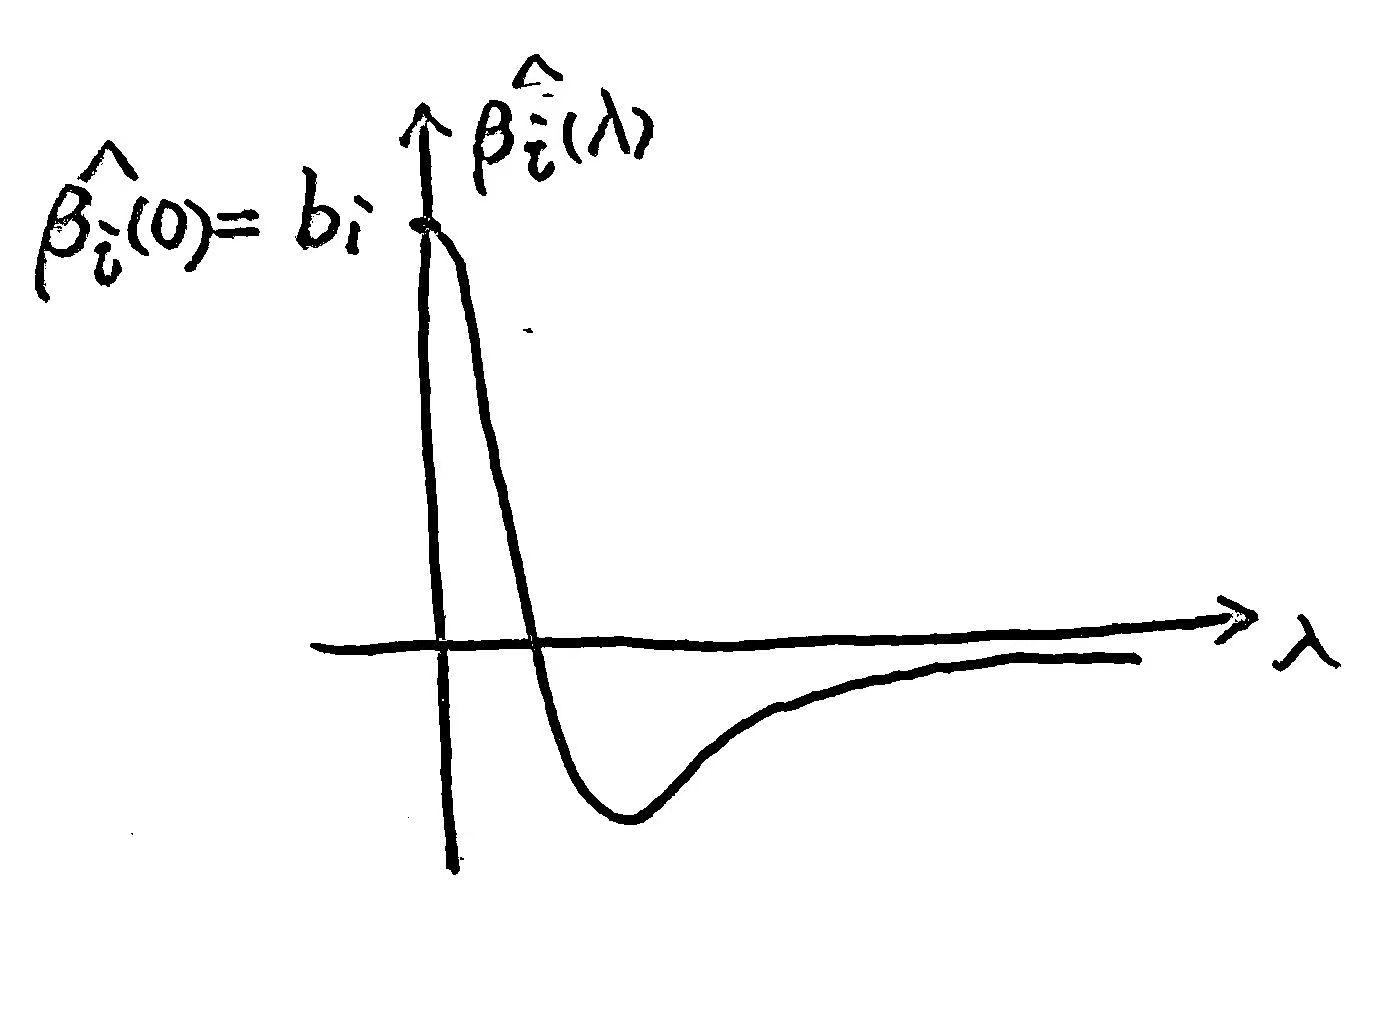
\includegraphics[width=0.8\textwidth]{figure1.jpg}
        \caption{岭迹图示例 1}
        \label{fig:figure1}
    \end{figure}
    
    \subsection*{② Figure 2}
    
    如图所示,最小二乘估计量 \(\hat{\beta}\) 的分量不显著,因此从标准多元线性回归的观点来看,解释变量 \(X\) 的解释作用不显著。但是 \(\hat{\beta}\) 的岭迹图显示:随着 \(k\) 增大,在相当长的区间内稳定为离零较远的负值(虽然我们知道它最终会趋于零)。因此从岭回归的观点来看,解释变量 \(X\) 的解释作用显著。这说明在本例中,标准多元线性回归没有反映真实情况。
    
    \begin{figure}[h]
        \centering
        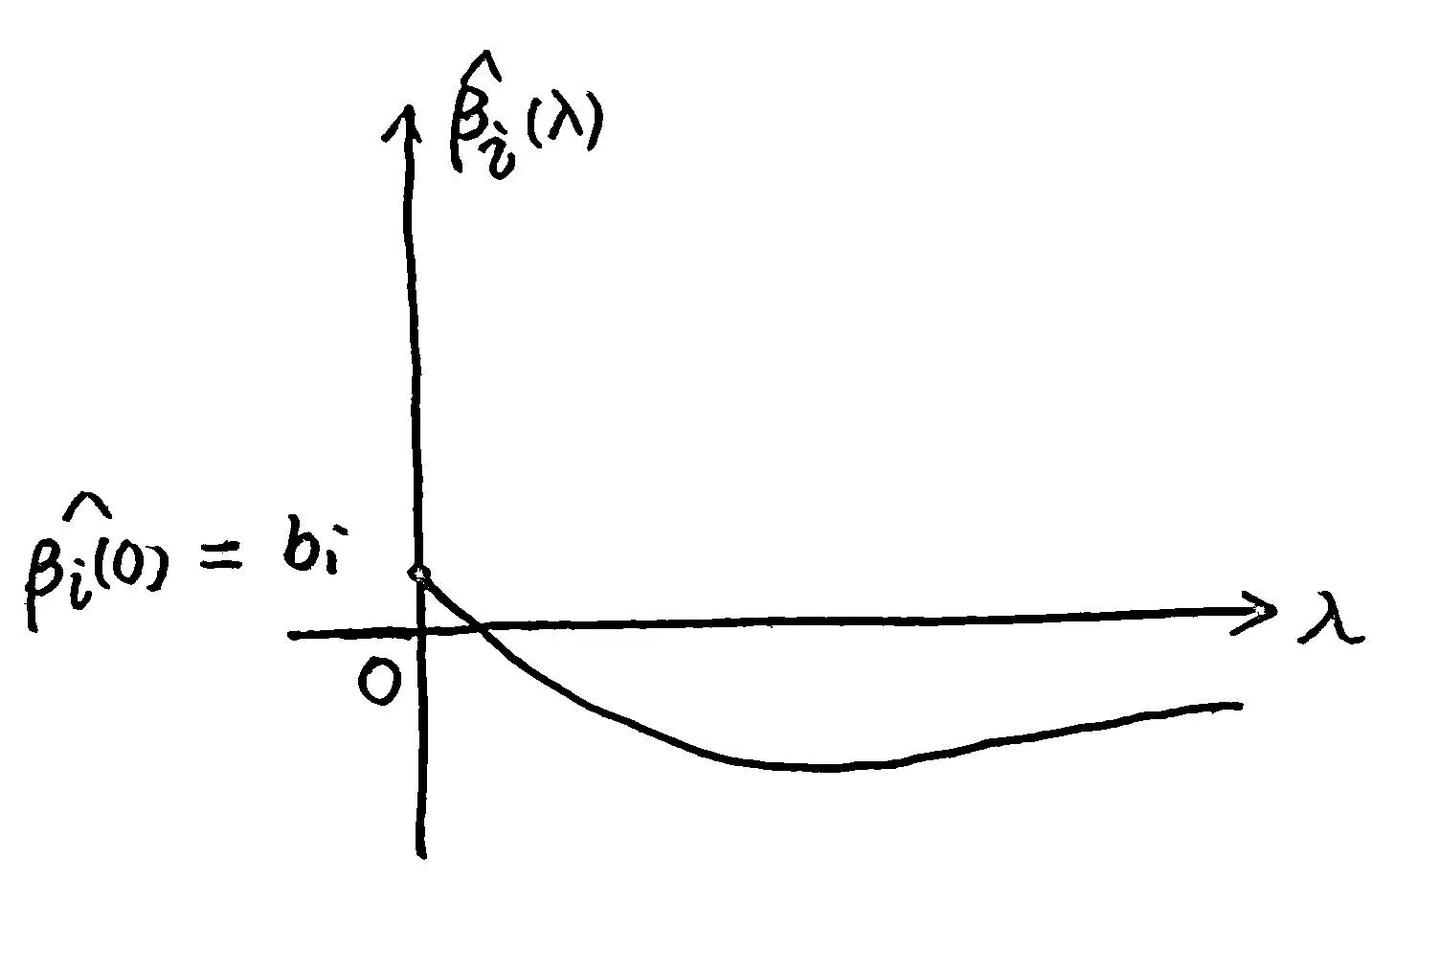
\includegraphics[width=0.8\textwidth]{figure2.jpg}
        \caption{岭迹图示例 2}
        \label{fig:figure2}
    \end{figure}
    
    \subsection*{③ Figure 3}
    
    如图所示,我们发现 \(\hat{\beta}_1\) 和 \(\hat{\beta}_2\) 的岭迹曲线都很不稳定,但它们的线性组合 \(\hat{\beta}_1 + \hat{\beta}_2\) 却相当稳定。这说明解释变量 \(X_1\) 和 \(X_2\) 之间存在多重共线性。
    
    \begin{figure}[h]
        \centering
        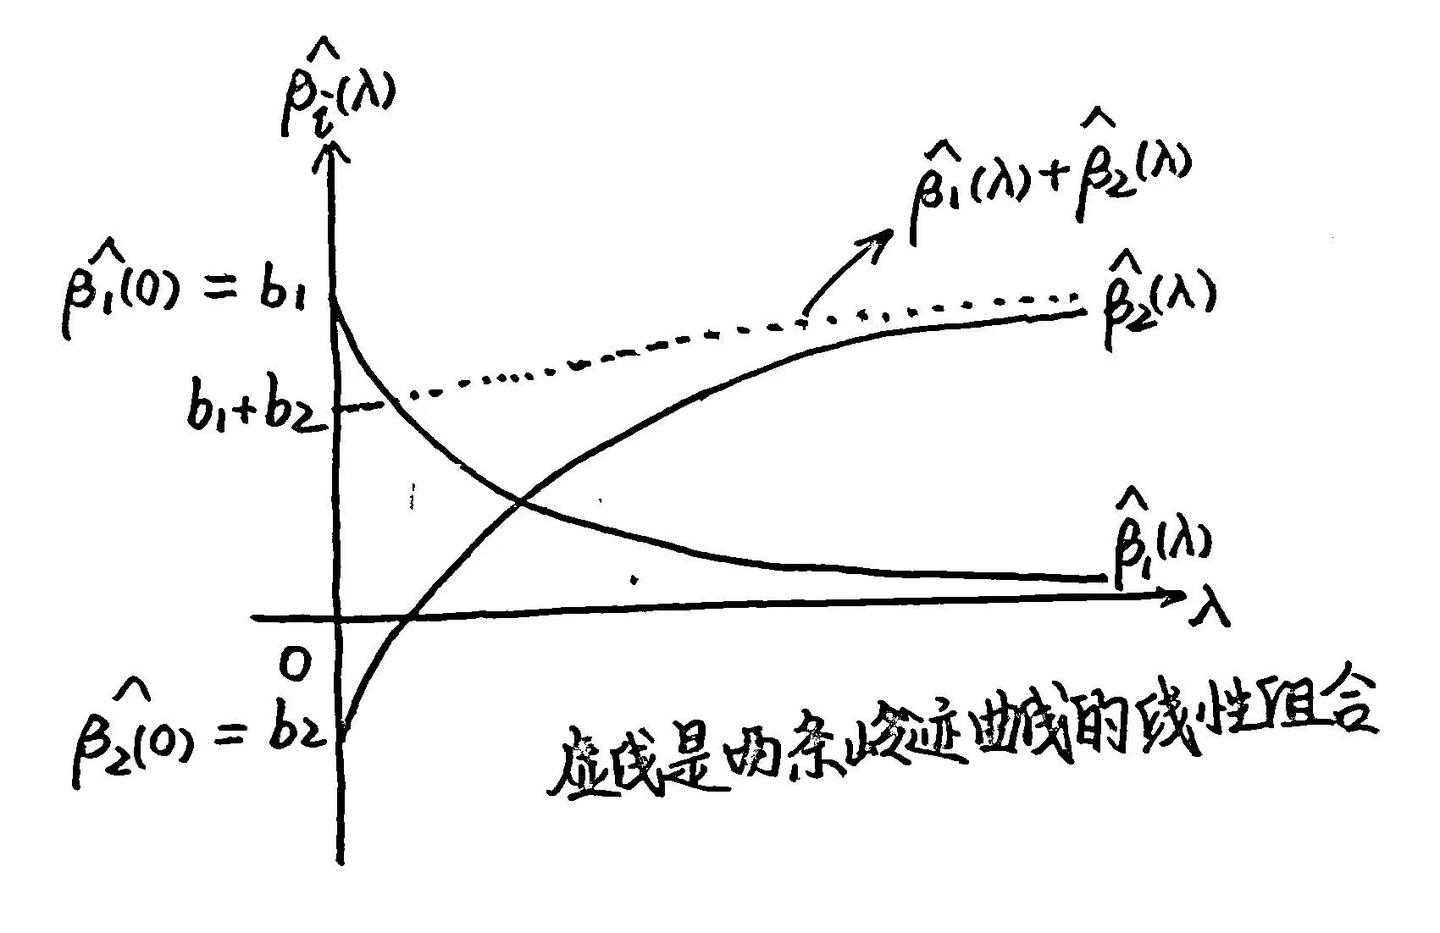
\includegraphics[width=0.8\textwidth]{figure3.jpg}
        \caption{岭迹图示例 3}
        \label{fig:figure3}
    \end{figure}
    
    \subsection*{岭迹分析的全局视角}
    
    从全局来看,岭迹分析可用于判断标准多元线性回归对某一实例是否适用。我们将所有回归系数的岭迹曲线绘制在一张图像上。如果这些岭迹曲线的不稳定性很强,即整个图像呈现比较“乱”的局面(如图4-1所示),那么我们倾向于认为标准多元线性回归是不适用的。此时,我们应该使用岭回归,并选取合适的岭参数 \(k\)。反之,则认为标准多元线性回归是适用的(如图4-2所示)。
    
    \begin{figure}[h]
        \centering
        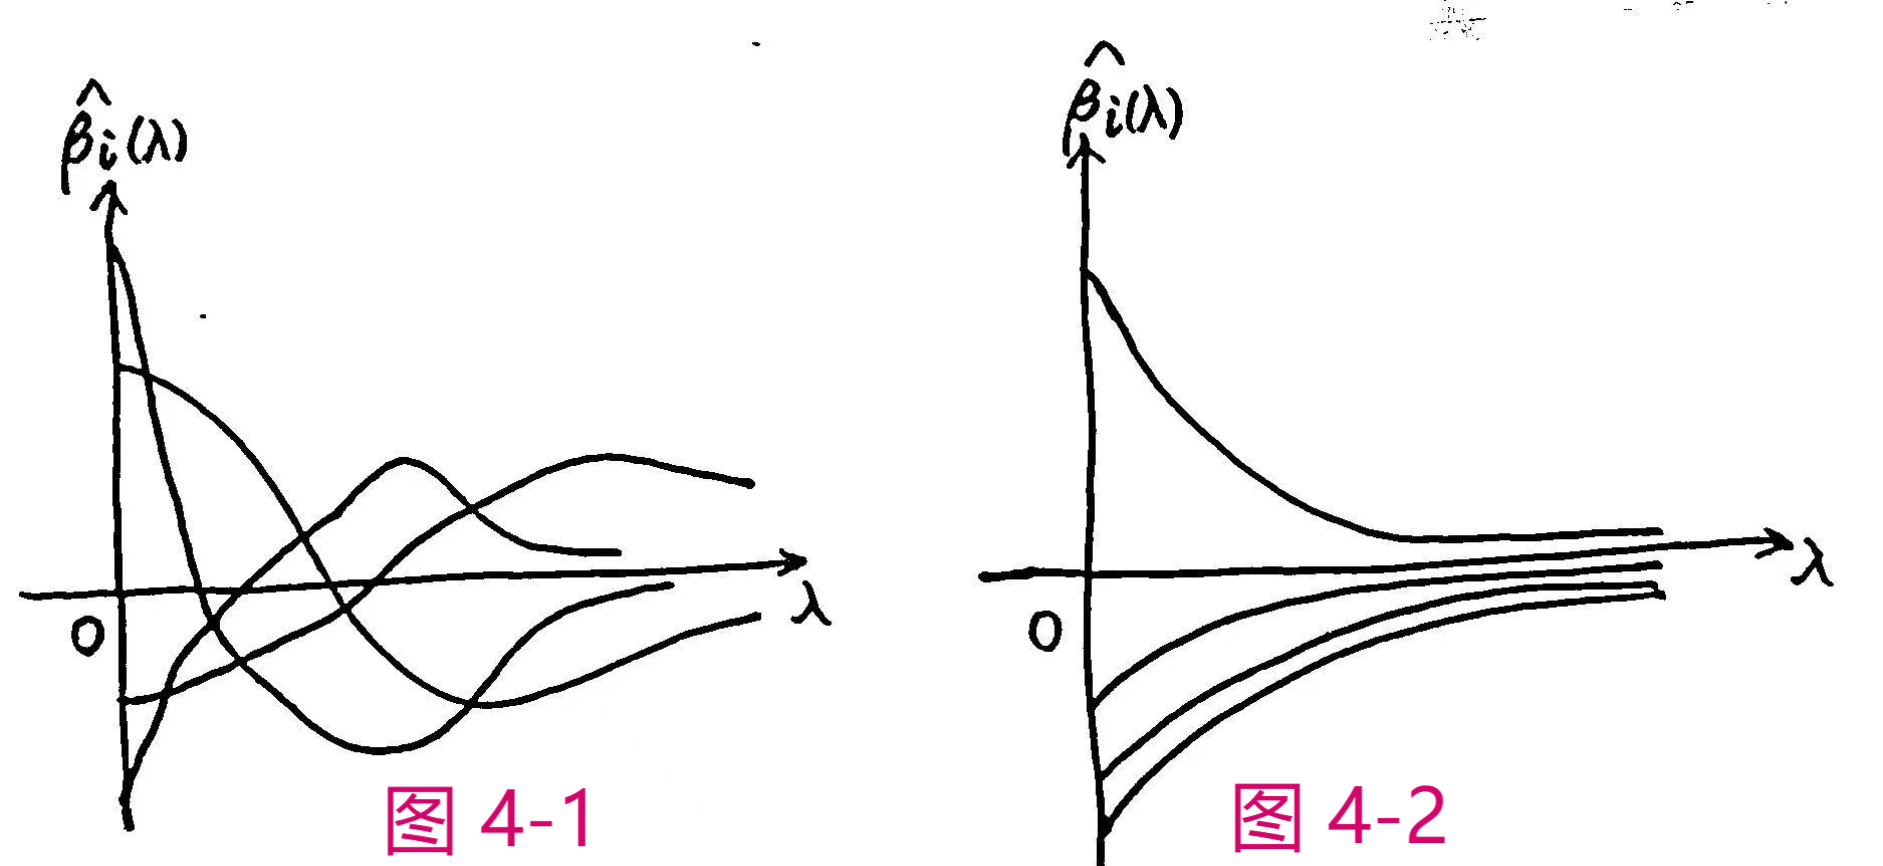
\includegraphics[width=0.8\textwidth]{figure4.png}
        \caption{岭迹图示例 4-1(不适用标准多元线性回归)4-2(适合)}
        \label{fig:figure4_1}
    \end{figure}
    
    
    
    \subsection*{岭参数 \(k\) 的选择}
    
    \subsubsection*{(1) 岭迹法 (Ridge Trace Method)}
    
    岭迹法的直观考虑是:如果标准多元线性回归的最小二乘估计量 \(\hat{\beta}\) 有不合理之处,那么我们希望通过采用适当的岭估计量 \(\hat{\beta}(k)\) 来获得一定的改善,其岭参数 \(k\) 的选取尤为重要。选取 \(k\) 的一般原则是:
    
    \begin{itemize}
        \item \(k\) 附近各回归系数 \(\hat{\beta}(k)\) 的岭估计量基本稳定;
        \item 分量的符号和绝对值与问题的实际意义相符;
        \item \(k\) 与 \(k\) 相比不增加太多。
    \end{itemize}
    
    具体的例子如图所示:我们发现 \(k\) 附近各回归系数的岭估计量基本稳定,因此我们可取 \(k\)。
    
    \begin{figure}[h]
        \centering
        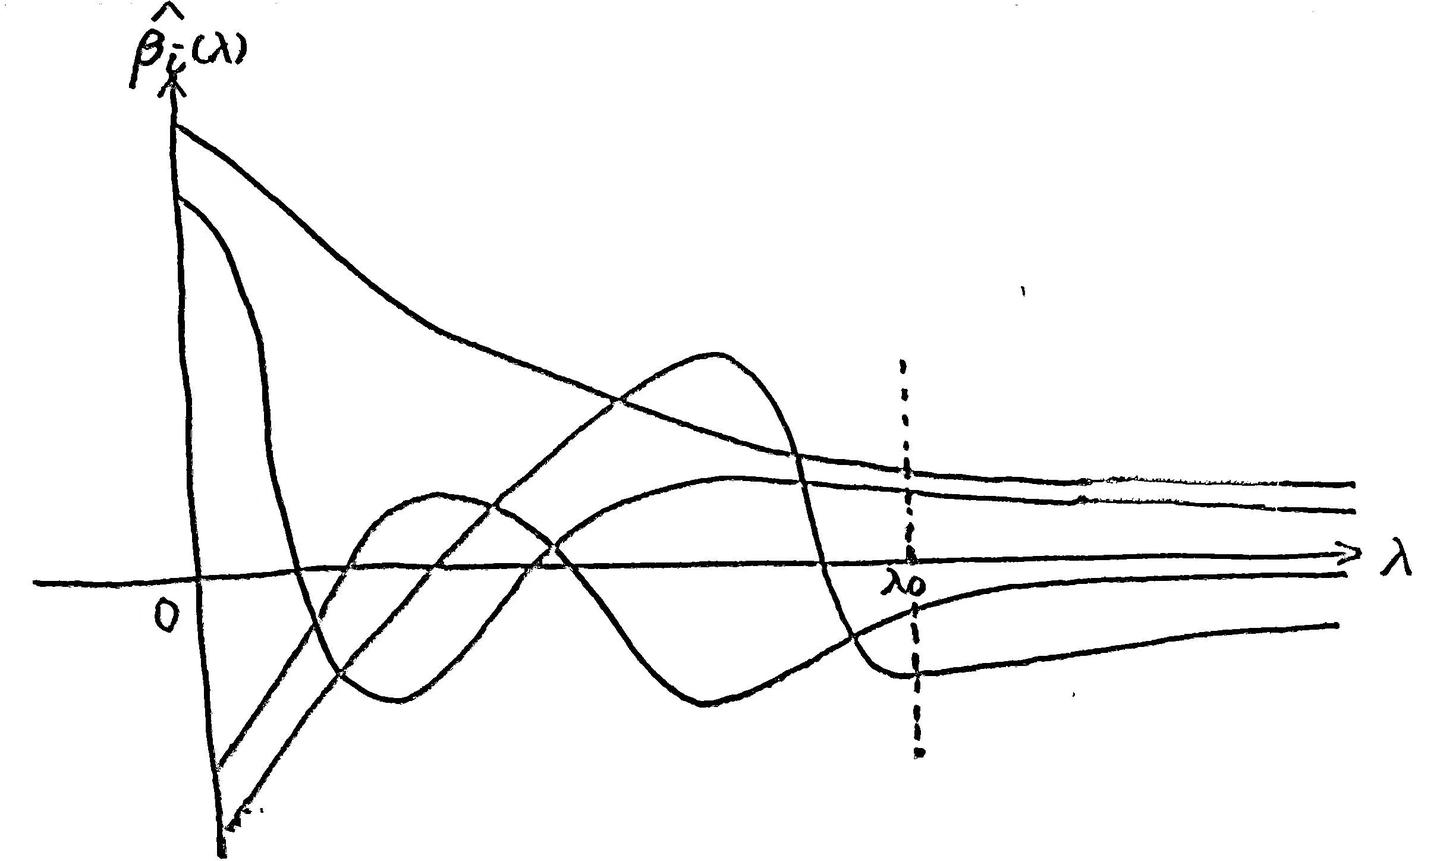
\includegraphics[width=0.8\textwidth]{figure5.jpg}
        \caption{岭迹图示例 5}
        \label{fig:figure5}
    \end{figure}
    
    值得注意的是,岭迹法与传统的基于残差的方法相比,其确定岭参数 \(k\) 的方法存在一定主观性,且缺乏严格的理论依据。我们可以将其作为一种定性分析,与后文所述的定量分析相辅相成。


        \end{document}